\documentclass[titlesmallcaps, examinerscopy, copyrightpage]{uqthesis}

\bibliographystyle{customIEEEtran}

\usepackage[usenames,dvipsnames]{color}
\usepackage[square,comma,numbers,sort&compress]{natbib}
\usepackage{pdfpages}
\usepackage{graphicx}
\usepackage{eurosym}
\usepackage{appendix}
\usepackage{play}
\usepackage[grey,times]{quotchap}
\usepackage{makeidx}
\makeindex
\usepackage{hyperref}
\usepackage{listings}
\usepackage[nottoc,numbib]{tocbibind}
\usepackage{verbatim}
\usepackage{amsfonts}
\usepackage{array}
\usepackage[acronym,nomain,nonumberlist]{glossaries}
\usepackage{listings}
\usepackage{setspace}
\usepackage[linewidth=1pt]{mdframed}
\usepackage{sverb}
\usepackage{bookmark}
\bookmarksetup{
  numbered, 
  open,
}

\makeglossaries
\renewcommand*{\glossaryentrynumbers}[1]{}

\newcommand{\tick}{\checkmark}
\newcommand{\gtick}{\color{ForestGreen} \tick }
\newcommand{\cross}{$\times$ }
\newcommand{\rcross}{\color{red} \cross }
\newcommand{\runz}{\textsc{Runz}}

\begin{document}
% =====================================================================
% =====================================================================
%%%%%%     TITLE
% =====================================================================
% =====================================================================

\hypersetup{pageanchor=true}
\pdfbookmark{Title}{toc}

\title{Undergraduate Thesis\\ \vspace{0.5 cm} ``Automatic and Assisted Redshift Analysis of Astronomical Objects" }
\author{Samuel Hinton}
\department{EAIT}

\renewcommand{\degreetext}{in partial fulfilment of the Degree Bachelor of Engineering\\ in the
discipline of Software Engineering}

\frontmatter

\titlepage



% =====================================================================
% =====================================================================
%%%%%%     FRONT CONTENT
% =====================================================================
% =====================================================================

\begin{flushright}
Samuel Hinton\\ 41966855\\ 78 Pegg Road, Rocklea, QLD 4106\\
\end{flushright}

\noindent \today \\

\noindent Prof Paul Strooper\\
Head of School\\
School of Information Technology and Electrical Engineering\\
The University of  Queensland\\
St Lucia QLD 4072\\

\noindent Dear Professor Strooper,\\ \\
In accordance with the requirement of the Degree of Bachelor of Engineering (Honours) in the School
of Information Technology and Electrical Engineering, I submit the following thesis entitled:

\begin{center}
  \emph{``Automatic and Assisted Redshift Analysis of Astronomical Objects''}
\end{center}

\noindent The thesis was performed under the supervisor of Dr Vaughan Clarkson and Dr Tamara Davis. I declare that the work
submitted in thesis is my own, except as acknowledge in the text and footnotes, and has not been
previously submitted for a degree at the University of Queensland or any other institution. \\

\noindent Yours sincerely \\ \\ 

\noindent \line(1,0){250} \\

\noindent Samuel Hinton

% =====================================================================

\chapter{Acknowledgements}

I would like to thank my supervisors, Tamara Davis, Vaughan Clarkson and Chris Lidman for their help, assistance and guidance throughout this thesis. I would also like to thank David Parkinson, Conor O'Neill, Michael Childress, David Lagattuta, Syed Uddin, Fang Yuan, Jeremy Mould, Richard Scalzo, Anthea King, Bonnie Zhang and Karl Glazebrook for their feedback, suggestions and testing during this thesis.

% =====================================================================

\chapter{Abstract}

I AM THE ABSTRACT


\cleardoublepage
\hypersetup{pageanchor=true}
\pdfbookmark[chapter]{Table of Contents}{toc}
%\addcontentsline{toc}{chapter}{Table of Contents}

\tableofcontents
\listoffigures
\listoftables

%\printglossary[title=Glossary]
%\addcontentsline{toc}{chapter}{Glossary}

\mainmatter


\chapter{Introduction}

Redshifting measurements form the backbone of many cosmological surveys, and in order to turn spectrographic measurements into quantified redshifts, a redshifting program is needed. In this thesis, the legacy redshifting software used by the OzDES cosmology team, \runz{}, is replaced with a new, web-based redshifting application developed specifically for their needs of high redshift and low signal-to-noise algorithms.\\

This report is divided into several sections, with the background and context for redshifting established in Chapter \ref{ch:back} and prior implementations discussed in Chapter \ref{ch:prior}. Those familiar redshifting and prior approaches are recommended to read from Chapter \ref{ch:req} or Chapter \ref{ch:design}, where program requirements and the implementation results are respectively discussed.



\chapter{Background}
\label{ch:back}

\section{Usefulness}

Redshifting a spectra is the process by which the degree of spectra from its original emission state is quantified. Over cosmic distances, the expansion of the universe causes travelling light to become stretched, and thus the measured amount of stretching provides valuable information about the travel time of the light, and thus the distance to the emission entity. As multiple cosmological models are still being actively considered \cite{davis2007scrutinizing}, it is prudent to keep measurements in the form of redshifts, as different cosmological models will translate redshifts to different comoving distances.\\

Redshifting can be obtained both from spectrographic and photometric data, each with advantages and disadvantages. Whilst photometric data can be used for fainter objects than currently viable for spectrographs, photometric redshifts do not possess the accuracy of spectrographic measurements \cite{bolzonella2000photometric}. It is important to note that the OzDES team, for which this thesis was undertaken, are not utilising any photometric redshifts as priors, nor does their instrumentation require photometric data. The OzDES team are utilising the Anglo-Australian Telescope (AAT) with the AAOmega spectrograph \cite{d2014ozdes}, and thus only require a spectrographic redshifting solution.

\section{Spectrographic Features}

Spectrographs provide accurate redshifting due to prominent discernible features in light emissions for galactic objects, where abundant elements such as Hydrogen, Nitrogen and Carbon either emit or absorb at different frequencies. Provided a high enough signal-to-noise ratio in a spectra, these peaks and troughs can be identified as potential features. Provided a sufficient amount of features, and they can be matched to known atomic transitions, whereupon the observed feature wavelength and the known feature wavelength can be combined to determine the redshift of a spectra. Figure \ref{fig:emission} provides a visual example of a high signal-to-noise spectra of the Seyfert 2 galaxy NGC 1068 (M77).

\begin{figure}[ht!]
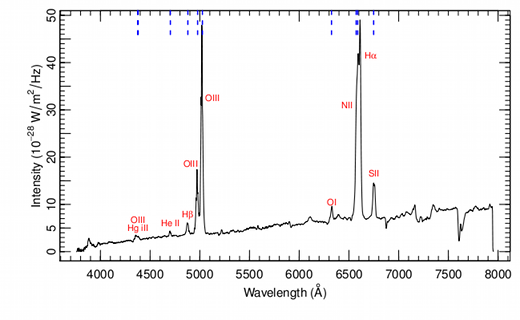
\includegraphics[width=0.75\textwidth]{images/M77_opt_spectrum.png} 
\centering
\caption{A plot of the emission from NGC 1068, with data from the NASA/IPAC Extragalactic Database\cite{nasaDB} and plot courtesy of public R code published by Alastair Sanderson \cite{emission}.}
\label{fig:emission}
\end{figure}

\section{Common Complications}

High quality spectra, with well defined and multiple emission features, such as shown in Figure \ref{fig:emission}, become progressively less common with increasing redshift, due to increasing distance to emission object and thus lower light intensity. As such, redshifting algorithms have to employ data reduction and matching techniques specifically designed to marginalise potential error and account of known complications. In this section, several complications to the redshifting process that have been actively encountered in this thesis will be discussed. Ideas on how to marginalise or reduce these complications will be discussed in the implementation section of this thesis.

\subsection{Planetary Atmospheric Interference}

Given that the Anglo-Australian Telescope is located on the ground in Australia, interference from the night sky has to be dealt with. The sky itself, possessing both necessary ingredients of light and atoms, has its own emission spectrum which all spectrographs will detect \cite{Meinel1950Emission}. By observing the night sky without a background source, the night sky can be subtracted out of target spectra, however this process can be imperfect in implementation due to spectrograph error and optical distortion \cite{Kelson2003Optimal}. Figure \ref{fig:night} shows the night sky spectrum above Mauna Kea.

\begin{figure}[ht!]
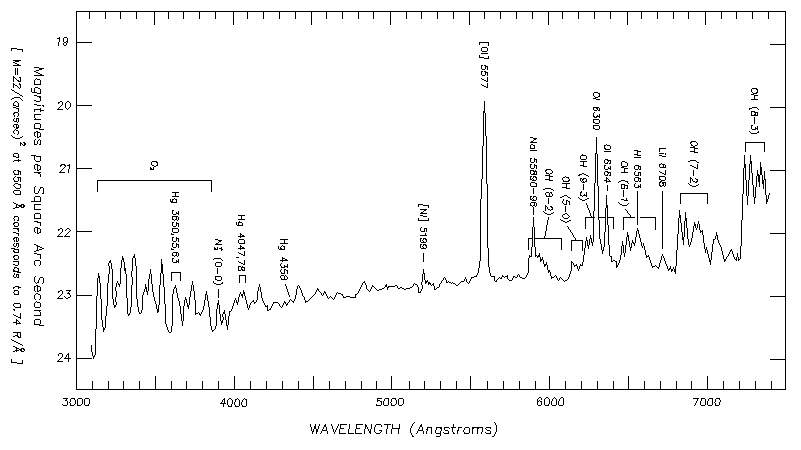
\includegraphics[width=0.75\textwidth]{images/om-nskyvis.jpg} 
\centering
\caption{A plot of the night sky emission above Mauna Kea from the Canada-France-Hawaii Telescope Observatory Manual \cite{night}. Please see the manual for data sources and further attribution.}
\label{fig:night}
\end{figure}

\subsection{Planetary Atmospheric Correction}

A simple consideration when examining spectra is that the wavelengths being recorded are the wavelengths of light in air (for a ground based telescope). Due to the complicated nature of converting air wavelengths to vacuum wavelengths, this is often done via interpolating conversions from empirical tabular data sets \cite{morton1991atomic}.

\subsection{Heliocentric velocity}

With the accuracy of spectrographic redshifting, the planet's heliocentric velocity provides a significant enough contribution that it needs to be corrected for \cite{colless20012df,baldry2014galaxy}. This can be done by calculating the relative velocity of the Earth in its solar orbit relative to the object being observed, and subtracting the appropriate redshift contribution.

\subsection{Cosmic Rays}

Cosmic rays are the name given to extremely high energy particles travelling in space. Cosmic rays are generally massive particles such as protons moving at relativistic speeds, often due to acceleration in a supernova \cite{ackermann2013detection}. Due to their colossal energy, in which the record is approximately $3\times10^{8}$ TeV (23 million times as energetic as the maximum energy rating of the Large Hadron Collider when set to reopen in 2015 \cite{lhc}), a single strike by a cosmic ray will appear as an extraordinarily thin and powerful emission line in a spectrum. Difficulty arises in filtering out cosmic ray strikes, but not filtering out emission lines, as the two features are similar in a spectra. The effect of a cosmic ray in a spectrum can be seen in Figure \ref{fig:cosmic}, where the massive peak near 5700{\AA} is a cosmic ray and not a true feature.


\subsection{Equipment Miscalibration}

Most modern spectrographs, including the AAOmega spectrograph, feature more than one charge-coupled device (CCD) with which to measure a spectrum \cite{aaomega}. Different CCD's are more sensitive to different wavelength ranges of light, and so in order to expand the wavelength range of the devices, CCD's with different range sensitivities are used. Problem can arise when trying to merge the separate sensor results into a final spectrum, with the possibility of spectral arms (with different CCD's) being miscalibrated. Miscalibrating the relative strength of the CCD's can lead to dichoric jumps in the spectrum, which can be easily mistaken for emission features. A sample spectra has been provided for illustrative purposes, and the dichroic jump can be clearly seen at approximately 5800{\AA} in Figure \ref{fig:jump}


\subsection{Physical Interference}

Difficulties in redshifting spectra can also arise when physical interference in the spectra can remove or hide useful features. A prominent cause of this interference is intergalactic and intragalactic dust and particulate, which will interact with light and often result in absorption troughs in the measured spectra. Not only do these introduced features not belong to the object that is trying to be observed, these absorption features can remove useful matching features of the base object if the absorption occurs at the same wavelength region as the expected feature. An example of erroneous absorption features added to a spectra can be seen in Figure \ref{fig:dust}, particularly in the first and third broad peaks, centred around 4400{\AA} and 5500{\AA} respectively.




\begin{figure}[ht!]
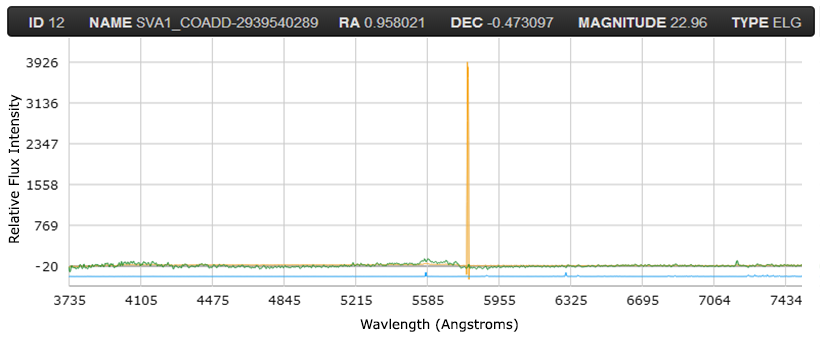
\includegraphics[width=1\textwidth]{images/CosmicRay.PNG} 
\centering
\caption{AAOmega spectrum of an emission line galaxy and a cosmic ray hit. Spectrum provided courtesy of Conor O'Neill and graphed using the developed thesis software prototype, with cosmic ray jump clearly visible at approximately 5700{\AA}}
\label{fig:cosmic}
\end{figure}

\begin{figure}[ht!]
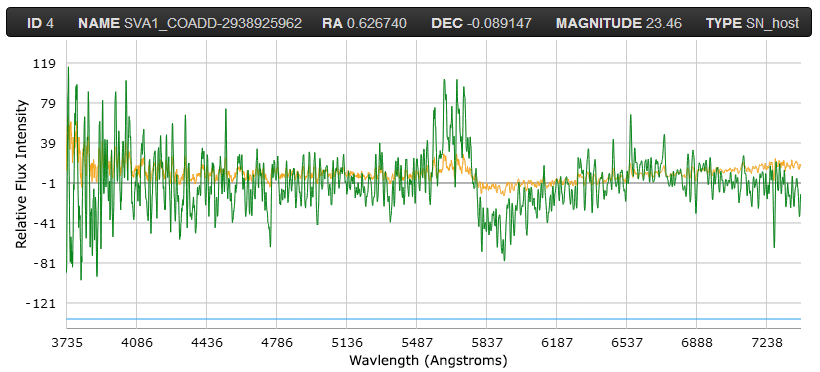
\includegraphics[width=1\textwidth]{images/jump.PNG} 
\centering
\caption{AAOmega spectrum of a supernovae host galaxy, spectrum provided courtesy of Conor O'Neill and graphed using the developed thesis software prototype, with dichroic jump clearly visible at approximately 5800{\AA}}
\label{fig:jump}
\end{figure}

\begin{figure}[ht!]
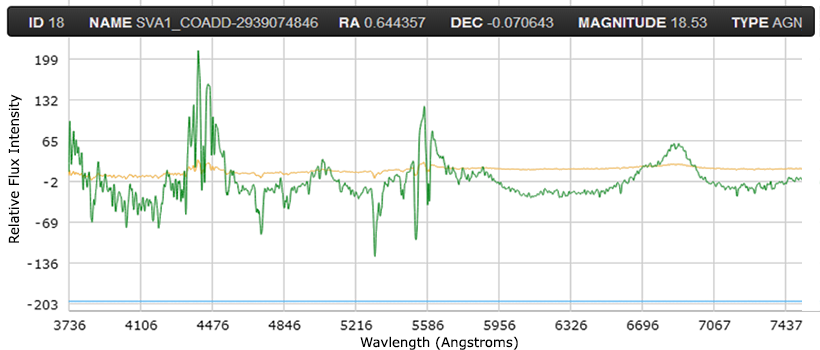
\includegraphics[width=1\textwidth]{images/dust.PNG} 
\centering
\caption{AAOmega spectrum of a quasar, spectrum provided courtesy of Conor O'Neill and graphed using the developed thesis software prototype, with erroneous absorption troughs scattered throughout the spectrum below from 4100{\AA} to 5900{\AA}.}
\label{fig:dust}
\end{figure}


\chapter{Prior Methods}
\label{ch:prior}

There are many prior approaches available for review, catering to a wide range of astronomical objects and varying observational distances and magnitudes. In this section, I will review several of the software packages used by large cosmology surveys.

\section{Implementations}

\subsection{RVSAO 2.0}

The RVSAO 2.0 software package is a highly used redshifting and templating software package, containing programs to perform cross correlation redshifting (\verb+xcsao+), feature matching (\verb+emsao+), template building (\verb+sumspec+) and more. The main program used for redshifting, \verb+xcsao+, is of main interest to this literature review, as the matching algorithm for the \verb+emsao+ program does not perform better in either high or low signal-to-noise spectra than \verb+xcsao+ \cite{kurtz1998rvsao}.

Power spectrum techniques were first used to analyse spectra by Tonry and Davis in 1979 \cite{tonry1979survey}, digitalising the analog techniques used by Griffin in 1967 \cite{griffin1967photoelectric}. The \verb+xcsao+ software program follows the methods outlined by Tonry and Davis, and has been in use since 1985 \cite{kurtz1998rvsao}. The specific algorithms of the \verb+xcsao+ program are outlined by Kurtz and Mink \cite{kurtz1998rvsao}, and are summarised below.

The software takes a spectrum with a user defined wavelength range, has continuum subtracted, and - depending on the configuration of the program - can also remove emission or absorption lines. The spectrum is then apodized to remove ringing in a Fourier transformation, zero-padded to remove potential artifacts after Fourier transformation, and then and Fourier filtered to try and improve the signal-to-noise ratio via a bandpass filter. The spectrum and each potential matching template is then rebinned, and cross correlated around a user defined redshift estimate to find the redshift of maximum correlation. The goodness of the fit is determined by the amount of main peak fit, and the final redshift and goodness are supplied to the user as the program's final result.

Whilst the cross correlation algorithms in use are tried and tested, the ease of use of the RVSAO 2.0 software package leaves much to be desired. Operating only in command line and without any interactive user input, the 2010 release of the \verb+xcsao+ program takes up to 67 input parameters \cite{parameters}, making intuitive use of the program impossible and introducing experience based technical overhead to cosmology groups attempting to use the software.

\subsection{2dF Galaxy Redshift Survey}
The 2dF Galaxy Redshift survey was designed to measure the redshift for approximately $250\;000$ galaxies using the Anglo-Australian Telescope \cite{colless20012df}. The algorithms used in the analysis of the spectroscopic data include data reduction and redshift estimation, where on the latter will be investigated in this review, as the data reduction pipeline used by OzDES is outside the scope of this thesis.

The matching algorithms used by the 2dF team are also descendent from the algorithms put forth by Tonry and Davis \cite{tonry1979survey}, where and, like RVSAO 2.0, redshift determination can be achieved both by cross correlation methods and feature matching \cite{colless20012df}. The spectrum given to the application first undergoes several steps of preprocessing, where detected atmospheric lines are removed via interpolation over a spectrum window. Continuum is removed via the subtraction of a fitted sixth degree polynomial, and points more than five times the root-mean-square (rms) deviation from the mean are removed from the spectrum. The spectrum is rebinned, apodized and then Fourier transformed. The transformed spectra is then filtered with an exponential filter to remove noise and subtract continuum further. The result of this filter is then cross correlated with all available templates, with the greatest cross correlation peak determining the final redshift.

Emission lines matching is done via fitting tight Gaussian peaks around strong emission features. The three strongest emission lines in the spectrum are tested against common strong emission lines, such as doubly ionized oxygen (O$_{\rm{III}}$), the hydrogen beta transition (H$_\beta$), the hydrogen alpha line (H$_\alpha$), or the double line from nitrogen (N$_{\rm{II}}$). If the emission lines are found to match these common transitions, the redshift can be determined via comparison of the detected peak wavelengths and the rest frame wavelengths.

After determining the final redshift, the spectrum is then displayed to the user, who then has the choice of accepting the suggested redshift or manually fitting the spectra themselves. The visual feedback provided by the 2dF software marks a large increase in usability over the RVSAO 2.0 software package.



\subsection{SDSS DR8 $\chi^2$ fitting}

The Sloan Digital Sky Survey (SDSS) has been active since 2000, and latest data release - data release 10, includes spectrographic measurements for over one million objects \cite{SDSSIII}. This review will concentrate on the eighth data release (DR8), in which the redshifting algorithms utilised are discussed more in depth. Prior to DR8, the redshifting algorithms used by the SDSS team included standard cross correlation techniques similar to those of 2dF and RVSAO 2.0, with $\chi^2$ algorithms also available \cite{sdss6}. In DR8, the cross correlation method was removed in favour of the $\chi^2$ fitting, as they gave the same results for approximately 98\% of spectra \cite{aihara2011eighth}.

The $\chi^2$ matching process is simpler than the cross correlation algorithm, and input spectra have a sky mask applied to zero weight skylines, and then, for a range of viable redshifts, the $\chi$ difference for each template in the catalogue is determined, where the $\chi^2$ difference is defined as:

\begin{equation}
\chi^2_z = \sum_i \left(\frac{t_{iz} - \mu_i}{\sigma_i} \right)^2,
\end{equation}

where the index $i$ denotes the $i$th data point, $t_iz$ is the value of the template's $i$th point at a shifted redshift of $z$, and $\mu_i$ is the value of the model's $i$th point. As of the eight data release, the redshift increment in each step is 138 km s$^{-1}$, and all galactic templates are checked between a redshift value of $-0.01$ to $1.00$. Whilst this method is certainly mathematically simpler than many alternate algorithms, the reviewer is concerned over the lack of detail given in the examined papers algorithm review about catering for factors such as varying normalisation over redshift ranges.



\subsection{\textsc{AUTOZ}}

The \textsc{AUTOZ} program written by Ivan Baldry is an IDL based algorithm to provide redshift estimation for the Galaxy and Mass Assembly (GAMA) team \cite{baldry2014galaxy}. In analysis of the matching algorithm, many similar steps to previously reviewed programs are found. \textsc{AUTOZ} applied flux corrections to account for non-uniform spectrographic sensitivity, removes bad data points, subtracts continuum via rejected polynomial fitting and subtraction of a smoothed median filter, apodizes the spectrum with a cosine taper and finally oversamples and rebins the spectrum. This final spectrum is then Fourier Transformed and cross correlated with a range of provided templates, where the highest cross correlation peaks are used to determine the best fitting redshift and template.

Unlike the 2dF program, which allows users to manually verify the automatically determined redshift and then pick their own redshift if unsatisfied, the \textsc{AUTOZ} program provides no interactivity or manual verification of redshifts. Whilst the program does allow a substantial number of input parameters to be specified that effects the matching algorithm, that is the extent of user input. Furthermore, the \textsc{AUTOZ} application is developed for a specific and restricted set of astronomical objects due to the target survey population of the GAMA survey.

\section{Trends and Caveats}

Given that the algorithms reviewed have been arranged in chronological order, it can be seen first off that emission line matching via feature identification has not been used in the more modern implementations. As discussed in the review of RVSAO 2.0, emission line matching has been found to be inferior to cross correlation matching for both high and low signal-to-noise data. Given the suitability of emission line matching mainly to high quality emission type galaxy spectra, this technique would be the least applicable to the low signal-to-noise survey being undertaken by the OzDES team.

When looking at cross correlation techniques, it can be seen that similarities in the matching algorithms of all four reviewed programs indicates that the core methodology has no changed significantly since it was first implemented by Tonry and Davis \cite{tonry1979survey}. The $\chi^2$ method of matching redshifts is only mentioned by the SDSS team, however they found it simple and useful enough to completely remove their cross correlation algorithms in favour of the $\chi^2$ approach. The success of that approach warrants an investigation and implementation of a $\chi^2$ matching algorithm in the thesis project, along with an implementation of a cross correlation based matching algorithm.


\section{Current OzDES Approach}

Currently the OzDES team is using legacy software called \textsc{Runz} to perform redshift estimates. This software provides two separate matching algorithms, respectively using cross correlation and feature matching similar to the RVSAO 2.0 software package. Similar to the 2dF software, the user can a manual redshift if unsatisfied with the best automatically determined redshifts. Users can find manual redshifts by virtue of marking spectral features as specific transitions via a simplistic visual interface illustrated in Figure \ref{fig:runz}, and can then perform a tightly constrained  automatic fit to shift the selection to the maximum cross correlation. The OzDES team is seeking replacement software due not only to the low accuracy of the automatic redshifting algorithm in \textsc{Runz}, but also due to the legacy nature of the software, which requires a Linux system to install, various dependencies, C-shell, in addition to a high learning curve. Modifying \textsc{Runz} to address these issues is not possible due to the unfortunate state of the code base after over a decade of revisions and additions. The next chapter will state the requirements of any replacement software in order to address the current disadvantages and issues relating to the installation and use of the current \textsc{Runz} software program.

\begin{figure}[ht!]
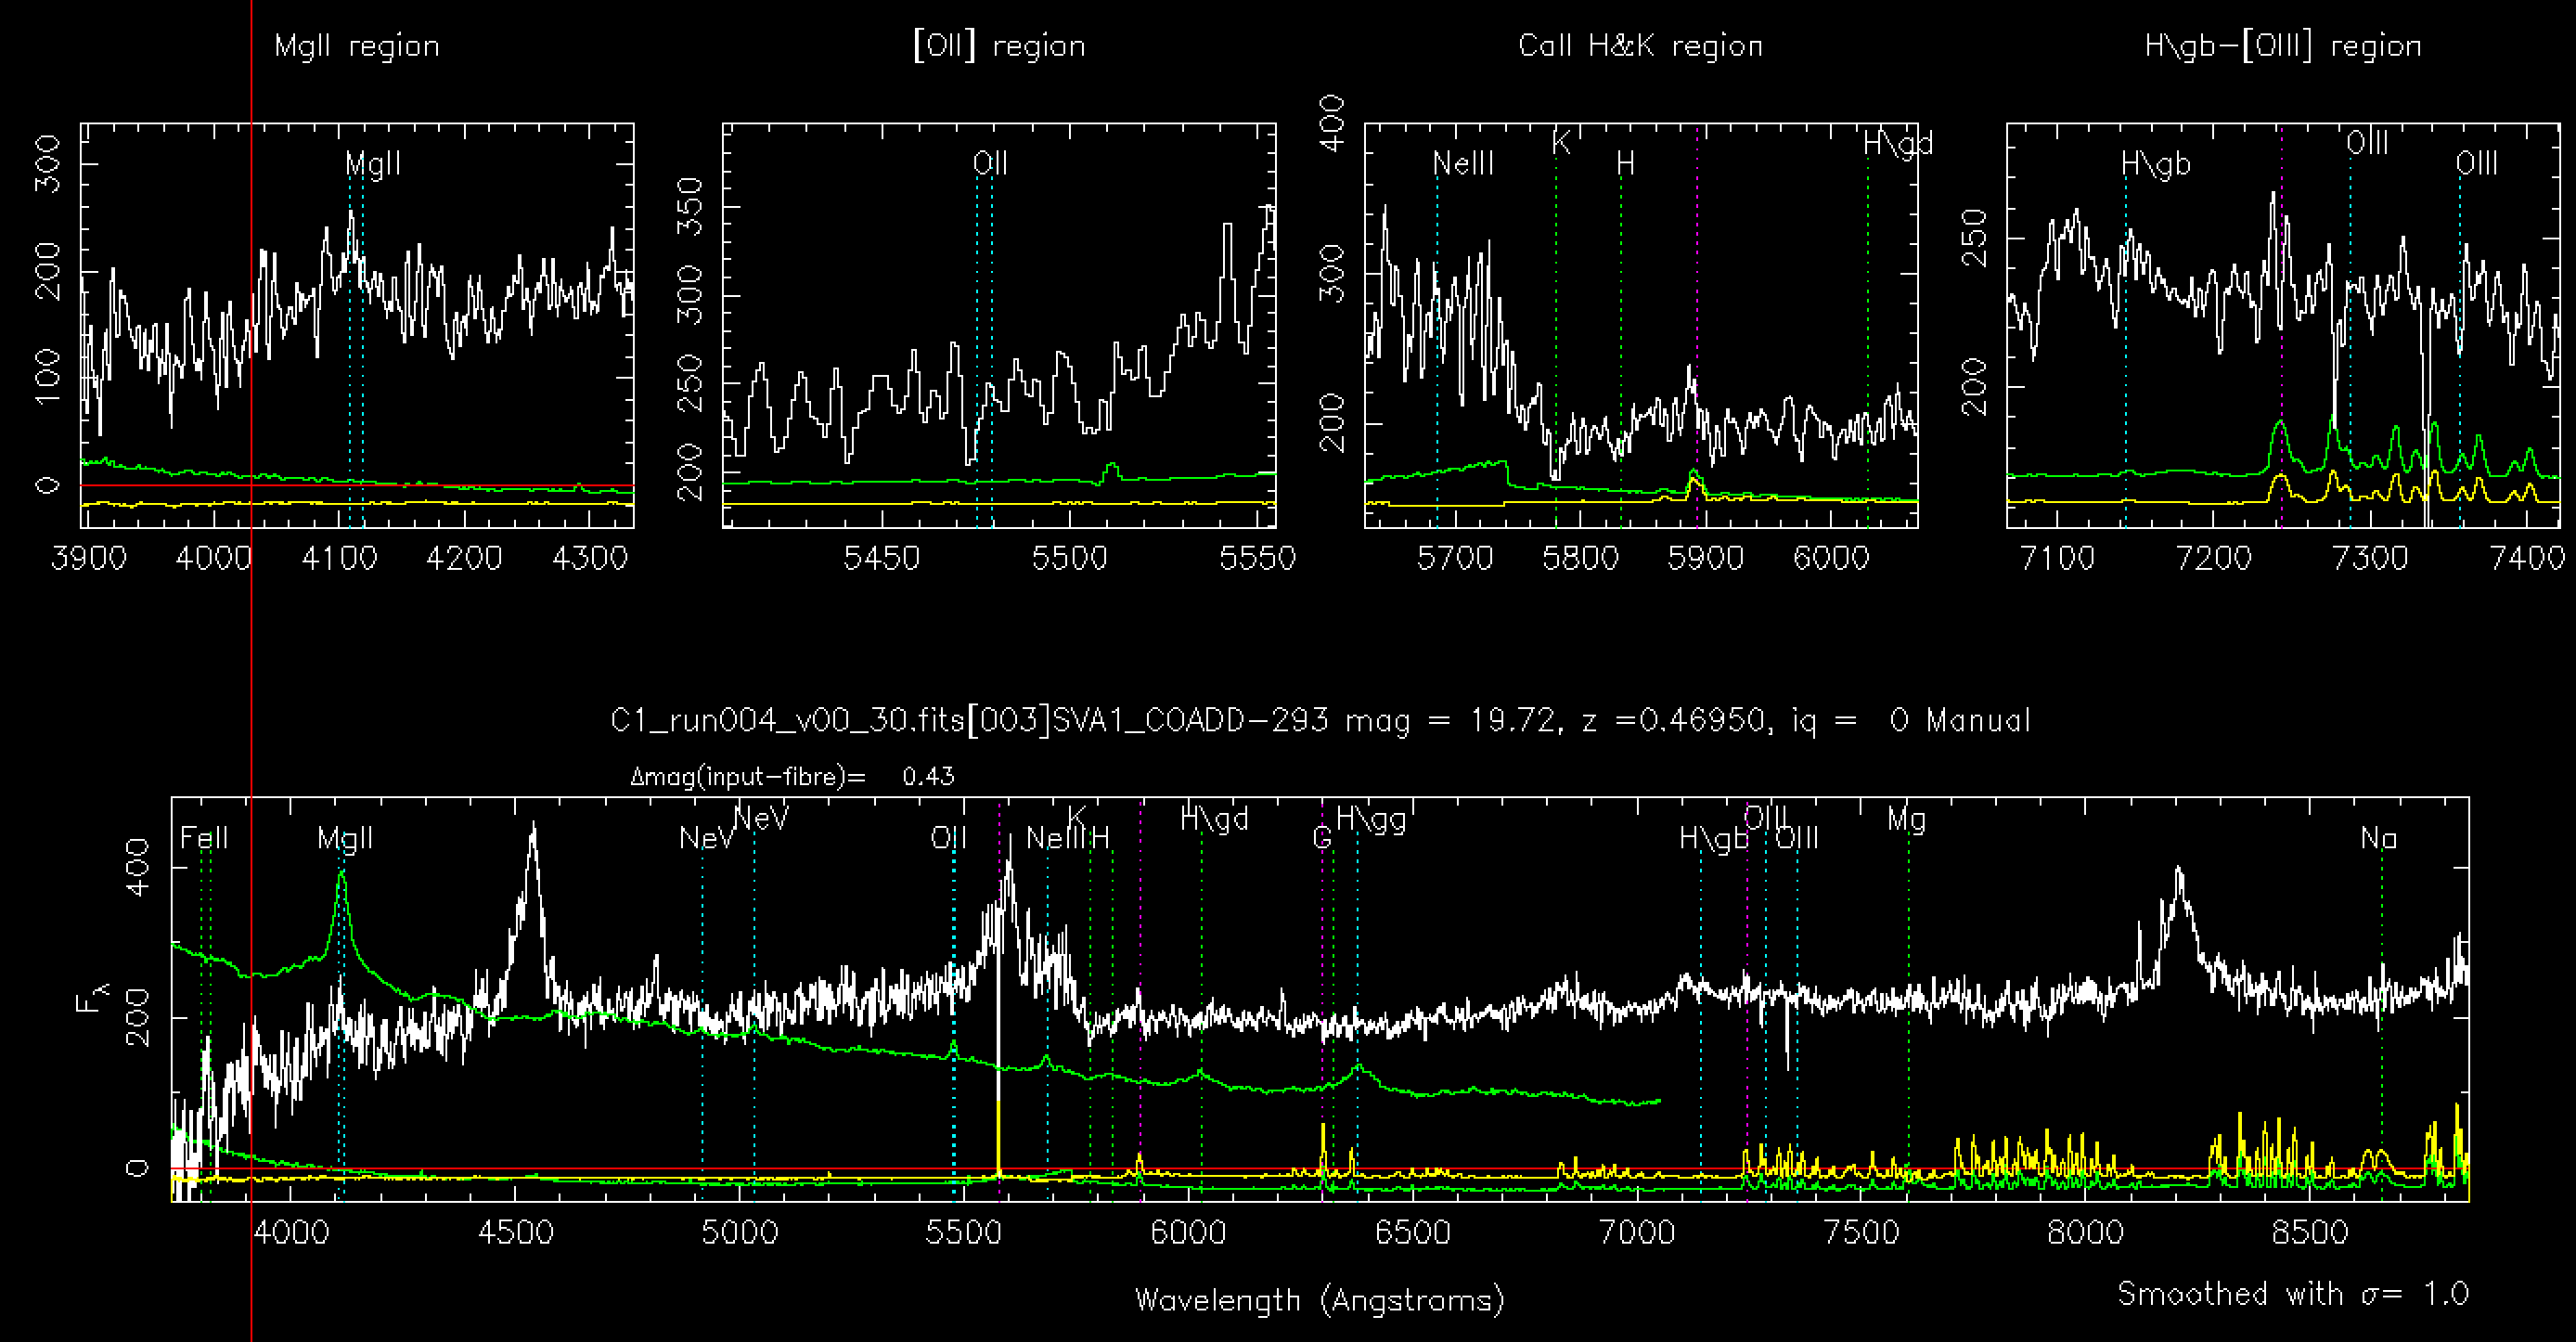
\includegraphics[width=1\textwidth]{images/RunzScreen.PNG} 
\centering
\caption{A screenshot of the \runz{} application in use. The four top plots represent detailed callout sections, with the full spectra shown in white in the bottom plot. The perspective template to match to is shown in green in all plots. The red line through the image serves as the cursor for \runz{}, where spectral lines are marked at the current cursor via keyboard shortcuts, which are displayed in a background terminal window to which \runz{} writes its output.}
\label{fig:dust}
\end{figure}



% =====================================================================

\chapter{Requirements}
\label{ch:req}

Consultation with the OzDES team produced a list of usability and functional requirements that need to be met before the thesis program can be considered a viable replacement for \textsc{Runz}. In this section, these requirements are discussed under the general categories of algorithm matching performance, computational performance, usability and integration features.
\section{Algorithm Performance}

Every night of observation at the AAT can produce four thousand spectra. Each of these spectra needs to be analysed by a member of the OzDES team to ascertain two values: a redshift estimate and a quality of estimate, as represented an integer range from 1 (illegible spectra) up to a quality of 4 (99\% confidence in results). The desired goal for the algorithm matching performance is to be able to agree with manual matching for 90\% of spectra, where the user has selected a quality of matching to be 4, indicating a high quality spectra and defined spectral features. Whilst other surveys and their matching algorithms have managed to attain over 90\% accuracy prior to this thesis, the algorithms developed for OzDES will need to be able to perform under circumstances of much lower signal-to-noise than previous surveys.

The absolute lower bound for accuracy during redshift estimate is to match the performance of the \textsc{Runz} application. Thus, analysis of algorithm performance will necessarily involve comparison to the performance of automatic matching via \textsc{Runz}.

Specifically, performance is looked to be gained in the area of quasar matching, which is a known weakness in prior algorithms and \textsc{Runz}, due to the high redshift estimations and broad features of quasar spectra. Generalising this requirement, any developed matching algorithm has to give high performance over a wide variety of traditional and exotic astronomical objects.

\section{Computational Performance}

The software developed needs to be accessible to end users without the aid of dedicated cluster or supercomputer stations. Memory and CPU utilisation of the application should fit within acceptable bounds such that the application can be executed without issue on computer hardware featuring dual core processors and 2GB of RAM. This is a soft goal, in that it is desired by not necessary for software adoption, however great care needs to be taken to ensure that the vast majority of expected users possess the hardware required to run the program without issue.

\section{Usability}

\subsection{Installation}

Given the legacy state of the current OzDES redshift matching software, \textsc{Runz}, initial installation of the software program and its required dependencies is an onerous task, and has taken in some cases over a week of effort before the program was in a usable state. A requirement for adoption by the OzDES would be significant improvements in the installation process. Ideally, installation should be achieved by a self-contained  single-file installation package, with any required dependencies installed either automatically or with minimal fuss.

Whilst cross-platform support is not a requirement for the OzDES team, it would be a desirable feature, as previous applications required a a Mac or Linux distribution.

\subsection{Updating}

In line with the request for minimal maintenance and human intervention, a further goal of this thesis will be to produce software that updates either automatically, or via a simple prompt to the end user. It is expected that at no point in any update process would a user have to manually updated any dependencies, or manually configure or replace program content, such as binary files.

\subsection{Uptake}

A final large issue that effects new users to \textsc{Runz} is the steep learning curve of the program. As briefly mentioned previously, \runz{} features a simple visual interface. This interface consists of cursor tracking, plot rendering and keyboard shortcuts, with none of the modern hallmarks and interactivity the define modern user interfaces. Furthermore, keyboard shortcuts, program output and help text is all displayed in a separate terminal window, creating an unpleasant disjoint between information location and the respective visual detailing of that information on the plots. The lack of modern control schemes and unintuitive segregation of information and visual content makes \runz{} unintuitive for new users, and the OzDES team are looking for an interactive and intuitive user interface in replacement software.

In addition to the usability of the interface in general, \runz{} provides limited screen options, restricting users to viewing a spectrum in full (as shown in Figure \ref{fig:runz}), or to seeing a plot detailing redshifts for all spectrum in the input file. It provides no way to inspect template files by themselves, no options or settings screen, and no overview screen by which to view multiple spectra, either in tabular or graphical format.

\subsection{Automation}

Although not a strict requirement, members of the OzDES team have enquired about the potential to automate the program, so that it can be inserted in the data pipeline without hassle. Given that manual data checks will still need to be performed, this requirement is an attempt to reduce time spent gathering relevant data files and waiting for the algorithm to redshift spectra before manually verifying the automatic results. As such, an objective for the algorithm is to match at a speed greater than that of a user manually matching spectra, to ensure that users do not find themselves waiting upon automatic matching to determine a redshift estimate.

\subsection{Retention}

The final usability requirement given by the OzDES team was to ensure that work could not be lost accidentally during the redshifting process. \runz{} achieves this goal via saving results straight to hard disk during redshifting, and similar levels of data retention need to apply for any developed application such that unexpected failure of the application, either through internal exceptions or being accidentally closed by the user, does not result in lost data and having to re-redshift spectra.




\section{Integration}

The final requirement for the program is in being able to integrate with the existing systems in place used by the OzDES team. Specifically, the program would need to take inputs of singular observation runs after data reduction, and be able to take data files created by aggregation of multiple observations by the OzDES team. The results produced by the program then need to be a consistent, machine readable format, suitable for easy digestion into a database system.



\chapter{Design Decisions}
\label{ch:design}

The requirements discussed in the previous chapter allow comparison of multiple possible development pathways. In this section, high level design decisions are laid out in terms of their advantages and disadvantages. 

\section{Languages}

\subsection{Python}

Python is a versatile, open-source, high-level programming language that supports the programming paradigms of object-orientated, structured, dynamic, functional and procedural coding \cite{Python}. It is gaining popularity quickly in the astronomical community, with 50\% of respondents to an astrostatistic survey specifying Python as their programming language of choice as of 2014 \cite{PythonPop}.

\subsubsection{Advantages}

\begin{itemize}
\item \textbf{External Libraries:} The greatest advantage of Python is the abundance of  high quality external python libraries available for academic use. In particular, the Astropy library provides programmers with a massive amount of relevant scientific methods, data analysis tools and data visualisation tools that can enormously simplify workflow processes \cite{astropy}. Other libraries, such as NumPy, focus on bringing speed to Python via wrapping compiled FORTRAN or C++ code in a Python wrapper, aiming to leverage the easy programming of Python with the efficiency of low-level languages \cite{numpy}.

\item \textbf{Platform agnosticism:} Python is available cross platform, and thus a Python implementation would be platform agnostic provided that any external libraries that use precompiled binary wrappers have versions available both unix based operating systems and Windows.

\item \textbf{Readability:} A final advantage of using the Python language is it's readability. Given that it is expected that multiple people will maintain the project and potentially contribute to it in the future, it would be highly beneficial if code written is easy to understand by readers without an in-depth technical background.
\end{itemize}
  

\subsubsection{Disadvantages}

\begin{itemize}
\item \textbf{Dependency Management:} Unfortunately, the large number of available Python libraries can often lead to dependency conflicts, where specific libraries require different versions of Python to work. In addition to this, a Python version chosen for the project would need to be installed onto all user's computers (as Python is interpreted), and some users may be reticent to installing a different version of Python for a single application.

\item \textbf{Advanced User Interface:} Whilst there are dozens of graphical user interface (GUI) libraries written for Python \cite{PythonGUI}, it is often the case that these libraries are platform dependent or require large amounts of code to create interactive interfaces. Given the thesis developer's inexperience with the most modern Python GUI, additional time would have to be devoted to selecting the best library available and learning how to us it.

\item \textbf{Updating:} Automatic updating would be difficult with a Python application in the circumstance of attempting to upgrade dependencies. As users may be utilising application dependencies for other projects, it is impermissible to update dependencies without notifying the user. In the case where other programs require a different version of an external library, unless the user decides to create a new Python installation, they cannot update the project.

\end{itemize}

\subsubsection{Verdict}

Despite the issues relating to external dependencies and unfamiliarity with developing Python user interfaces, the fantastic libraries available make Python a promising pathway to consider.


\subsection{C++}

C++ is a low-level, compiled programming language that is known for library support and high-speed execution \cite{cpp}.

\subsubsection{Advantages}
\begin{itemize}

\item \textbf{Speed:} Given that C++ is a low-level, compiled language, its execution speed is significantly faster than interpreted languages like Python. Given the numerical complexity and large data sizes found in many astronomical tasks, the speed of C++ can be required for high performance domains. Whilst this is obviously a boon in any circumstance, it should be noted that this project does not strictly posses an efficient high-performance computing requirement, and that many libraries in Python (such as NumPy) to some extent negate the speed benefit of C++.

\item \textbf{Maturity:} C++ is a mature ISO-standard language, and thus code written for C++ is highly likely to remain standards compliant over future revisions. As a counter example to this, consider the fragmentation in the Python code base which is split between versions 2.7.8 and 3.4.1 due to large code changes \cite{pythonDownload}.
\end{itemize}

\subsubsection{Disadvantages}
\begin{itemize}

\item \textbf{Fewer Modern Libraries:} Given the low popularity of C++ in astronomy, regularly updated and comprehensive libraries are few and far to be found. Whilst general scientific and signal processing libraries exist, the list of high quality C++ libraries pertaining to astronomy libraries is not as comprehensive as available in Python. In addition, many C++ libraries are platform dependent, locking down platform choices.

\end{itemize}

\subsubsection{Verdict}
In light of the fact that the speed advantages of C++ over interpreted languages like Python are largely removed due to Python wrappers over compiled binaries, the only compelling reason to implement the program in C++ is unconvincing.


\subsection{IDL}

IDL is a programming language developed by Exelis specifically for scientific computing, aiming to be easy to use, easy to read, and concise \cite{idl}. 

\subsubsection{Advantages}
\begin{itemize}
\item \textbf{Built in functions:} Being a scientific computing language, IDL comes with a large amount of built in functions that lowers the requirement for external dependencies for complex mathematical functions, visualisation and data manipulation. Given the scientific context of IDL, it also has built in support for array operations not found in many other languages.
\item \textbf{External libraries:} IDL is still a common choice for astronomical projects \cite{PythonPop}, and this is in large part due to comprehensive astronomical library repository available from NASA \cite{IDLAstro}. These libraries, in addition to the base functionality in the IDL language, cover most common astronomy data analysis cases.
\end{itemize}
\subsubsection{Disadvantages}
\begin{itemize}
\item \textbf{Syntax:} For developers unfamiliar with IDL, the large changes in standard language syntax throughout the language vastly reduce the readability of the code. Unusual function declaration and signatures, variable handling, pseudo-classes are but a few of the syntax irregularities of IDL from common languages like C, C++, Java, Python and FORTRAN.
\item \textbf{Cost:} IDL requires a yearly license to install, which would discourage users to install the program onto personal computers instead of academic devices.
\item \textbf{Interface:} IDL is primarily a procedural programming language and as such as few scant GUI features. Whilst developing some form of interface is possible with IDL, the high levels of interactivity desired may be unattainable without low level implementation of the user interface, which is to be avoided at all costs.
\end{itemize}
\subsubsection{Verdict}

The price of IDL, its lack of proper interface support, and uncomfortable syntax easily outweigh the potential benefits of built in features and external libraries. As such, IDL cannot be recommended as the development language.

\subsection{Javascript}
\subsubsection{Advantages}
\begin{itemize}
\item \textbf{User Interface:} A Javascript computing program can leverage HTML and CSS interfaces, allowing the full range of functionality given by modern web pages with minimal effort. Javascript has hundreds of helper libraries designed to add to the base functionality of Javascript, and scores more to add better control between HTML and Javascript. This further reduces the difficulty of designing a high quality user interface.
\item \textbf{Platform agnosticism:} All that a Javascript application requires to run is a modern browser, which is already a requirement for the OzDES team with their internet-based database system. In addition to platform agnosticism, a Javascript application has no installation and updates on refresh of the page.
\item \textbf{Novelty:} Whilst not an advantage in terms of the OzDES team, scientific computing on a javascript application is highly unusual. This approach would therefore allow investigation of web applications as a basis for future scientific computing.
\end{itemize}
\subsubsection{Disadvantages}
\begin{itemize}
\item \textbf{Sandboxing:} Due to browser security, web applications are highly sandboxed. Access to the file system and system functions is impossible, and persistent storage is both browser specific and severely limited in size. 
\item \textbf{Lack of libraries:} Given the novelty of scientific computing in Javascript, there is a severe lack of proper libraries for either formal data analysis and astronomical functions. The lack of these libraries would lead to manual implementation of a large amount of extraneous functions that could be found pre-implemented in either Python, C++ or IDL.
\end{itemize}

\subsubsection{Verdict}

Whilst the sandboxing and lack of scientific libraries presents a difficult problem to overcome, the usability benefits, user interface benefits and especially the novelty of a javascript approach make it an extremely interesting avenue.


\section{Language Decision}

After analysis of the four proposed options of Python, C++, IDL and Javascript, the options of C++ and IDL can be safely discarded. Given the extra potential for unique research afforded by said novelty of the Javascript implementation, it was chosen over Python. However, due to the problems with the Javascript approach, and their inability to be solved (without changes to web security standards), a backup plan involving both Python and Javascript is kept in contingency. Such a plan could utilise a Python based local web server such as Django to perform the scientific analysis of the program if Javascript was unable to, and locally send the results to a Javascript interface via traditional HTTP requests and simplified via use of Representational State Transfer (REST), which allows implicit serialisation of Javascript objects to and from string representations that can easily be sent via the HTTP protocol. It is hoped that Javascript can be utilised for the entire application, and details on how the main issues with Javascript are to be avoided is provided in the next section.


\section{Frameworks and Libraries}

Due to the large number of frameworks, not all of them can be compared in this section. Instead, only the chosen frameworks will be examined.

\subsection{Angularjs}

Angulajs is a javascript framework designed by Google to allow HTMl, CSS and Javascript to interact in one Model-View-Whatever control scheme \cite{angularjs}. Two way data bindings between a Javascript model and HTML model would greatly simplify the creation of responsive user interfaces. Whilst other javascript frameworks exist, such as Ember.js and Backbone.js, none of them provide the utility and easy binding that angularjs can provide.

\subsection{jQuery}

jQuery is a javascript libraries aimed towards extending the native function of javascript, particularly in the area of HTML document manipulation, event handling and animation \cite{jQuery}. jQuery will be utilised in the project for the simplifications of manipulating DOM elements.

\subsection{Bootstrap}

Bootstrap is a collection of CSS styles and javascript helpers that allow easy creation of modern, flexible and responsive web interfaces \cite{bootstrap}. Bootstrap is being used to reduce the amount of time spent creating high quality interfaces.


\subsection{fitsjs}

Fitsjs is a javascript library that allows the reading of FITs files - the output format for astronomical files that will be used by OzDES that can include image data, binary tables, data cubes and more \cite{fitsjs}sar. The usage of the library should significantly decrease the amount of peripheral code required to be written before work can begin on the redshifting algorithms.


\chapter{Implementation}
\label{ch:impl}


\section{User Interface}


\section{Matching algorithm}


Talk about EVERYTHINGGGGGGG



\chapter{Project Evaluation}

\section{Completion}



\begin{table}[ht!]
	\center
	\begin{tabular}{c|c|c}
		\hline
		Feature & Complete & Incomplete \\
		\hline
		Surface Capture & \gtick & \\
		Human interface (Control Panel) & \gtick & full UI synchronisation between multiple clients \\
		External control interface (RPC) & \gtick & \\
		Configurable (JSON Keystore) & \gtick & More settings should be user configurable \\
		Real-time Computer Vision for \newline Block Diagram recognition & \gtick & \\
		Block Diagram Model output \newline (MQTT Publish/Subscribe) & \gtick & \\
		\ldots & & \\
		Digital Logic Adapter & & \rcross \\
		Minimalist Digital Logic Simulator & & \rcross \\
		\hline
	\end{tabular}
	\caption{Feature completion for BlocSim prototype}
	\label{tab:completion}
\end{table} 

\newpage
%\clearpage

\section{Performance}

Talk about performance

\begin{description}
	\item[Network] - For a 1080p image cropped to approximately 50\% of its width and height, the jpeg frame size after base64 encoding is approximately 60KB. At a nominal frame rate of 5FPS, this gives 2.4mbps bandwidth for video, which is quite manageable on local networks. A blocsim server intended for remote access over the web should be constrained to a lower frame rate using the UI controls.
	\item[CPU] - This has not been extensively tested. On a MacBook Pro Retina with a 2.4GHz i5 processor, 8GB RAM, and integrated Intel graphics, the server ran at approximately 70\% CPU usage with one client attached (local). This is acceptable for personal use on a modern middle-range computer. 
	\item[Frame Rate] - At a full 1080p on the above system, BlocSim was able to maintain image processing at the speed-limited 5FPS.
\end{description}


\section{Design Decisions}
\label{ch:review:design}

Talk about design decisions

\section{Future Improvement}

Talk about what could be done in the future.
% =====================================================================

\chapter{Conclusion}

 This is my conclusion




























\chapter*{References}
\begingroup
\addcontentsline{toc}{chapter}{References}
\renewcommand{\addcontentsline}[3]{}
\renewcommand{\chapter}[2]{}
\bibliography{IEEEabrv,bibliography}
\endgroup


% =====================================================================

\end{document}
